%!TEX root = ED_Grafo.tex

\section{Ordenamento Topológico}
\begin{frame}
	\begin{itemize}
		\item Ordenação linear de todos os vértices, tal que se $G$ contém uma 
		aresta $(u, v)$ então $u$ aparece antes de $v$.
		\item Pode ser vista como uma ordenação de seus vértices ao longo de uma 
		linha horizontal de tal forma que todas as arestas estão direcionadas da 
		esquerda para a direita.
		\item Pode ser usado sempre que o problema abordado envolve uma ordem parcial.
		\item Um grafo pode ter vários ordenamentos topológicos possíveis.
	\end{itemize}
\end{frame}

\begin{frame}[label=notas]
	\begin{columns}[T]
		\column{.5\textwidth}
			\begin{tikzpicture}[every node/.style={circle,draw},node distance=15mm]
				\node (7) {7};
				\node[below right of=7] (11) {11} edge[line,<-] (7);
				\node[above right of=11] (5) {5} edge[line,->] (11);
				\node[below left of=11] (2) {2} edge[line,<-] (11);
				\node[below right of=5] (8) {8} edge[line,<-] (7);
				\node[above right of=8] (3) {3} edge[line,->] (8);
				\node[below left of=8] (9) {9} edge[line,<-] (8) edge[line,<-] (11);
				\node[below right of=8] (10) {10} edge[line,<-] (3) edge[line,<-] (11);
			\end{tikzpicture}
			\pause
		\column{.4\textwidth}
			\begin{enumerate}
				\item 7, 5, 3, 11, 8, 2, 9, 10% (visual esquerda-para-direita, de-cima-para-baixo)
				\item 3, 5, 7, 8, 11, 2, 9, 10 %(vértice de menor número disponível primeiro)
				\item<1- | alert@3-> 3, 7, 8, 5, 11, 10, 2, 9%
				\item 5, 7, 3, 8, 11, 10, 9, 2 %(menor número de arestas primeirofirst)
				\item 7, 5, 11, 3, 10, 8, 9, 2 %(vértice de maior número disponível primeiro)
				\item 7, 5, 11, 2, 3, 8, 9, 10%
			\end{enumerate}
	\end{columns}
	\pause\vfill
	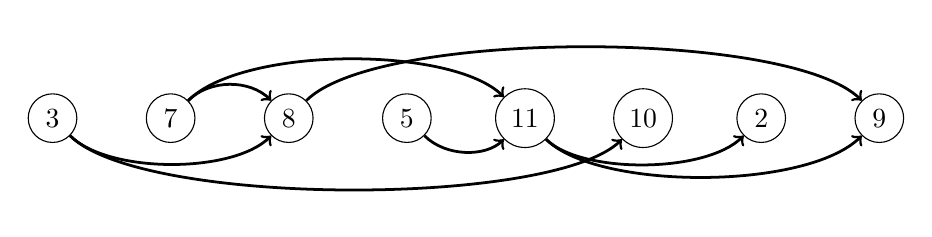
\begin{tikzpicture}[every node/.style={circle,draw},node distance=15mm]
		\node (3) {3};
		\foreach \x/\y in {7/3,8/7,5/8,11/5,10/11,2/10,9/2}
			\node[right of=\y] (\x) {\x};
		\foreach \x/\y/\z in {3/8/1,3/10/1.6,5/11/0.7,11/2/1,11/9/1.3}
			\draw[line width=1pt,->] (\x) ..controls +(south east:\z) and +(south west:\z) .. (\y);
		\foreach \x/\y/\z in {7/11/1.3,7/8/0.7,8/9/1.6}
			\draw[line width=1pt,->] (\x) ..controls +(north east:\z) and +(north west:\z) .. (\y);
	\end{tikzpicture}
\end{frame}

\begin{frame}[fragile]
	Algoritmo para Ordenamento Topológico:
	
	\begin{itemize}
		\item Adaptação da busca em profundidade.
		\item Durante a busca em profundidade, a cada vértice completo, insere na 
		frente de uma lista encadeada.
	\end{itemize}
	
	\begin{center}
		\begin{minipage}{.7\textwidth}
			\begin{lstlisting}[morekeywords={ord_top,v_node_t, processa, vizinho, processado, insere}]
			ordenamento_topologico(G)
				para cada vertice em V
				    g[v] := grau_de_entrada(v)
				    se g[v] = 0
				        insere(fila, v)
				    j := 0
				    enquanto !vazia(fila)
				        v := retira(fila)
				        insere(resultado, v)
				        j := j+1
				        para cada (v,u) em A
				            g[u] := g[u]-1
				            se g[u] = 0
				                insere(fila, v)
			\end{lstlisting}
		\end{minipage}
	\end{center}
\end{frame}

\begin{frame}
	\framesubtitle{Aplicação: Escalonamento}
	
	\pause
	\begin{block}{Escalonamento}
		Organização (distribuição e ordem de execução) de tarefas nos recursos disponíveis.
	\end{block}
	\pause
	Objetivos:
	\begin{itemize}
		\item Ser justo(evitando o adiamento indefinido).
		\item Maximizar a produtividade (\emph{throughput}.
		\item Ser previsível.
		\item Minimizar o tempo de resposta para usuários interativos.
		\item Maximizar o número possível de usuário interativos.
		\item Minimizar a sobrecarga (overhead).
		\item Balancear o uso de recursos.
		\item Exibir degradação previsível e progressiva em situações de intensa 
		carga de trabalho.
		\item Etc.
	\end{itemize}
\end{frame}

\begin{frame}[label=notas]
	\framesubtitle{Aplicação: Escalonamento}
	
	\begin{columns}
		\column{.35\textwidth}
			\begin{enumerate}
				\item Pegar ovo.
				\item Pegar o óleo.
				\item Untar a frigideira.
				\item Quebrar o ovo.
				\item Esquentar o óleo.
				\item Pôr o ovo na frigideira.
				\item Esperar o ovo fritar.
				\item Retirar o ovo.
			\end{enumerate}
		\column{.65\textwidth}
			\pause
			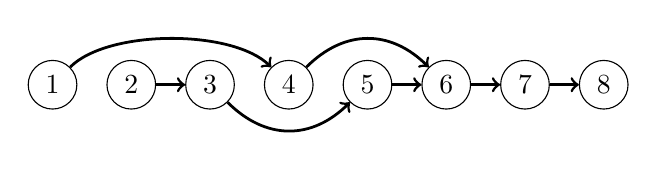
\begin{tikzpicture}[every node/.style={circle,draw}]%,node distance=2cm]
				\node (1) {1};
				\foreach \x/\y in {2/1,3/2,4/3,5/4,6/5,7/6,8/7}
					\node[right of=\y] (\x) {\x};
				\foreach \x/\y in {1/4,4/6}
					\draw[line width=1pt,->] (\x) ..controls +(north east:1) and +(north west:1) .. (\y);
				\foreach \x/\y in {2/3,5/6,6/7,7/8}
					\draw[line width=1pt,->] (\x) -- (\y);
				\draw[line width=1pt,->] (3) ..controls +(south east:1) and +(south west:1) .. (5);
			\end{tikzpicture}\\\vfill\pause
			\begin{tikzpicture}[every node/.style={circle,draw},node distance=13mm]
				\node (1) {1};
				\node[right of=1] (4) {4} edge[line width=1pt,<-] (1);
				\node[below of=4] (5) {5};
				\node[left of=5] (3) {3} edge[line width=1pt,->] (5);
				\node[left of=3] (2) {2} edge[line width=1pt,->] (3);
				\node[right of=4] (6) {6} edge[line width=1pt,<-] (4) edge[line width=1pt,<-] (5);
				\node[right of=6] (7) {7} edge[line width=1pt,<-] (6);
				\node[right of=7] (8) {8} edge[line width=1pt,<-] (7);
				\pause
				\node[rectangle, white, above right of=1] {\textcolor{greenUnB}{Recurso 1}};
				\node[rectangle, white, below of=3, above=3mm] {\textcolor{blueUnB}{Recurso 2}};
				\node[rectangle, white, above of=7, below=3mm] {\textcolor{redUnB}{Recurso ?}};
				\node[rectangle, dashed, line width=2pt, greenUnB, fit=(1) (4)] {};
				\node[rectangle, dashed, line width=2pt, blueUnB, fit=(2) (3) (5)] {};
				\node[rectangle, dashed, line width=2pt, redUnB, fit=(6) (7) (8)] {};
			\end{tikzpicture}
	\end{columns}
\end{frame}

% \begin{frame}
%	\frametitle{Componentes fortemente conectados}

%	Um componente contectado $C$ é o maior conjunto de vértices ${u, v} \in C$ 
%	tal que $u \leadsto v$ e $v \leadsto u$. 

%	\pause \vfill

%	\begin{block}{Aplicabilidade}
%		Uma quantidade significativa de problemas, aparentemente complexos,
%		são reduzidos a identificação ou contagem de componentes
%		fortementes conectados de um grafo.
%	\end{block}
% \end{frame}

% \begin{frame}[label=notas]
%	\frametitle{Exemplo (Fonte: Introduction to Algorithms)}

%	\begin{center}
%	
\includegraphics[scale=0.5]{stronglyConnectedComponents.png}
%	\end{center}
% \end{frame}